\section{Hilo de ejecuci\'on de un experimento}

La duraci\'on de un experimento puede ser de horas, esta caracter\'istica involucra tres problematicas
a resolver:

\begin{itemize}
    \item Evitar time-out del lado del cliente web.
    \item Desacoplar la atenci\'on de una petici\'on HTTP de usuario de la ejecuci\'on de un experimento.
    \item Lograr una experiencia de usuario agradable en lo que respecta a performance.
\end{itemize}

Modelando el proceso de ejecuci\'on con un hilo separado del principal es una soluci\'on
v\'alida para resolver el problema y teniendo en cuenta los siguientes:

\begin{itemize}
    \item Seguimiento del estado del hilo.
    \item Control sobre el numero de hilos creados.
    \item Gesti\'on de los datos durante la ejecuci\'on del hilo.
\end{itemize}

\begin{figure}[!htb].
    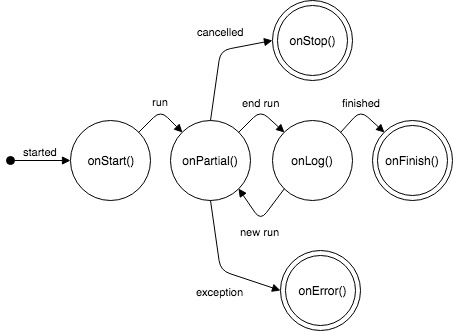
\includegraphics[width=\linewidth]{../figures/d14.jpg}
    \caption{Estados de un hilo de experiemento.}
    \label{fig:d14}
\end{figure}

\newpage